\subsection{Gráficos dos Cenários}

Os gráficos a seguir apresentam uma visão abrangente das projeções financeiras para um período de 12 meses, considerando os cenários pessimista, realista e otimista.

Na Figura \ref{cenarioRealista}, podemos observar que, em um cenário realista, a possibilidade de alcançar o ponto de equilíbrio ocorre em 10 meses, resultando em um lucro de R\$ 20.000 ao final do período de 12 meses.

Entretanto, a Figura \ref{cenarioPessimista} destaca o cenário pessimista do projeto, no qual não se vislumbra a capacidade de atingir o ponto de equilíbrio dentro do prazo de 12 meses, ocorrendo apenas próximo ao décimo terceiro mês de projeto, com um lucro de R\$1.217,00

Por último, a Figura \ref{cenarioOtimista} ilustra o cenário otimista do projeto, onde os lucros apresentam um crescimento mais rápido e o ponto de equilíbrio é alcançado mais cedo, precisamente em 9 meses e meio. Ao término dos 12 meses, é esperado um lucro de aproximadamente R\$ 25.000,00.

\begin{figure}[H]
    \center
	\caption{\label{fig_sge20}Gráfico do Cenário Realista}
    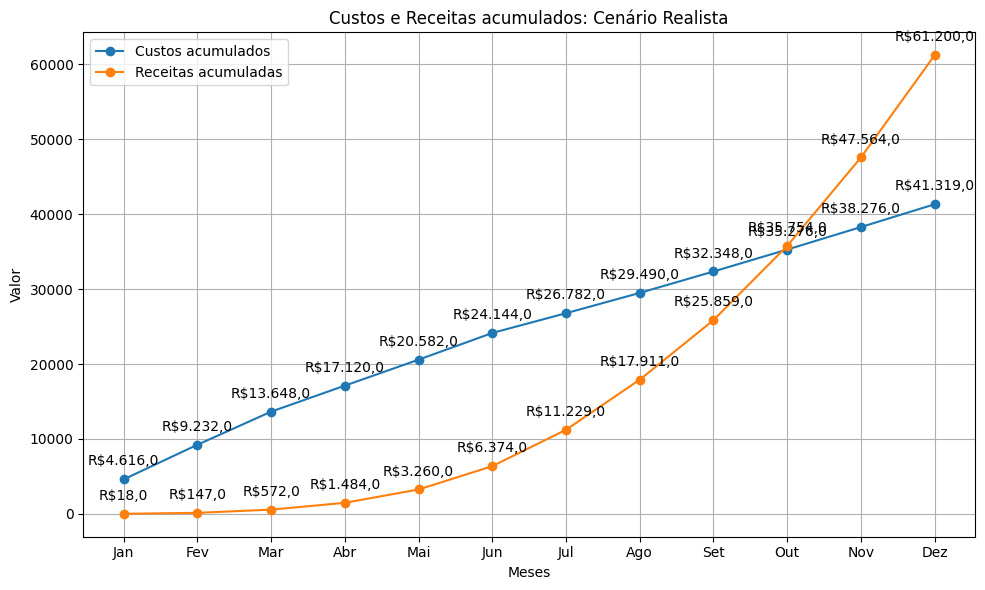
\includegraphics[scale=0.60]{imagens/viabilidadeFinanceira/Projeção-Receita_Custos-Realista.png}
    \label{cenarioRealista}
	\fonte{Os autores}
\end{figure}

\begin{figure}[H]
        \center
	\caption{\label{fig_sge20}Gráfico do Cenário Pessimista}
    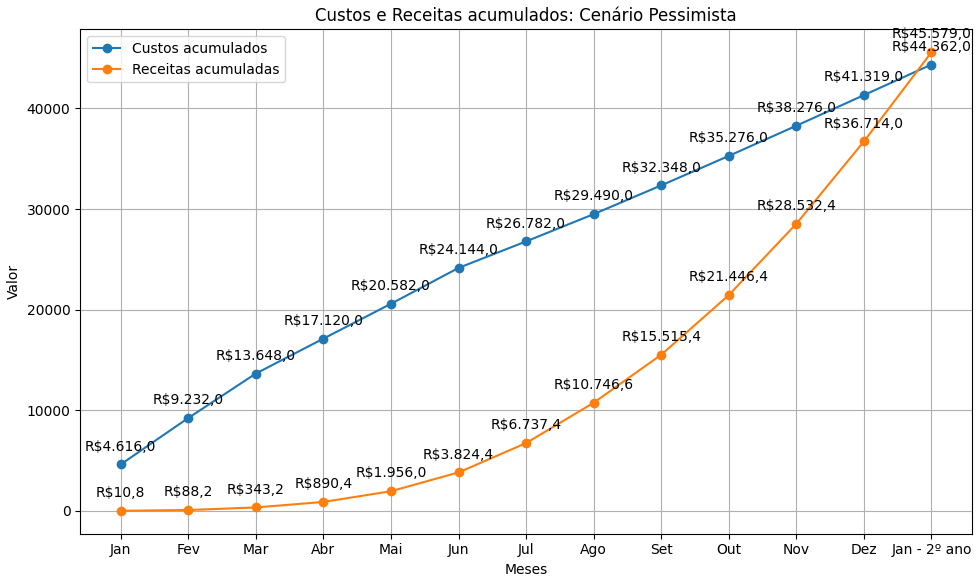
\includegraphics[scale=0.60]{imagens/viabilidadeFinanceira/Projeção-Receita_Custos-Pessimista.png}
    \label{cenarioPessimista}
	\fonte{Os autores}
\end{figure}

\begin{figure}[H]
        \center
	\caption{\label{fig_sge20}Gráfico do Cenário Otimista}
    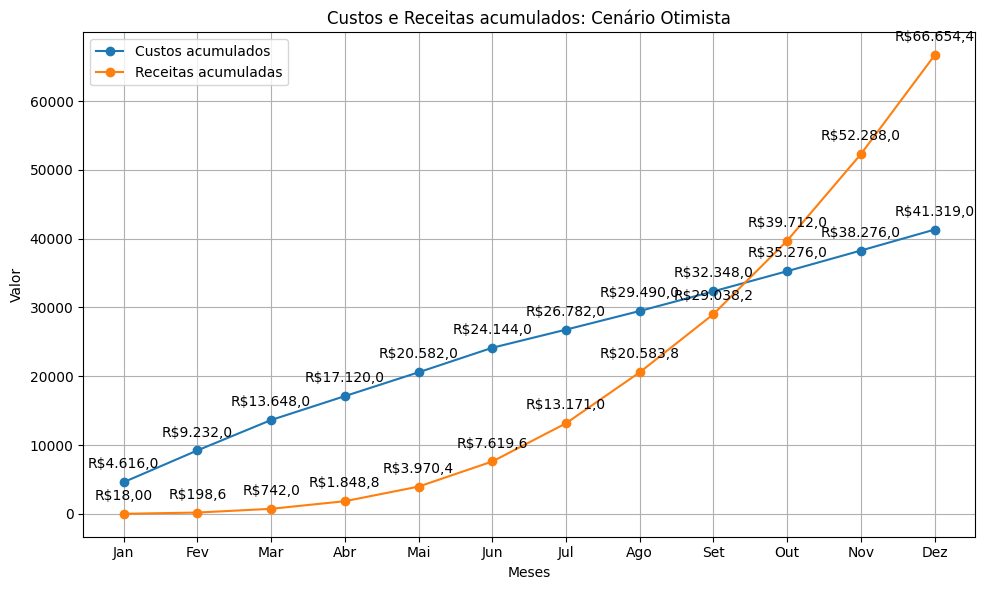
\includegraphics[scale=0.60]{imagens/viabilidadeFinanceira/Projeção-Receita_Custos-Otimista.png}
    \label{cenarioOtimista}
	\fonte{Os autores}
\end{figure}